% Define the document type and font size
\documentclass[12pt]{article}

\usepackage[spanish]{babel} % Package for the Spanish language
\usepackage[utf8]{inputenc} % Package for UTF-8 character encoding
\usepackage{geometry} % Package to configure document margins
\usepackage{listings} % Package to include source code in the document
\usepackage{xcolor} % Package to define colors
\usepackage{fancyhdr} % Package to customize headers and footers
\usepackage{amsmath} % Package for advanced mathematical symbols and environments
\usepackage{amssymb} % Package for additional mathematical symbols
\usepackage{graphicx} % Package to include graphics

\setlength{\parskip}{1em} % Space between paragraphs
\setlength{\parindent}{0pt} % Without indentation for paragraphs

% Definition of colors for source code
\definecolor{KEYWORDS}{HTML}{0000ff}
\definecolor{COMMENTS}{HTML}{888888}
\definecolor{STRINGS}{HTML}{ff0000}

% Configuration of the listings environment to display source code
\lstset{
	frame=shadowbox,
	language=c++,
	aboveskip=3mm,
	belowskip=3mm,
	xleftmargin=10mm,
	xrightmargin=10mm,
	showstringspaces=false,
	columns=flexible,
	basicstyle={\small\ttfamily},
	numbers=left,
	numberstyle=\tiny\color{COMMENTS},
	keywordstyle=\color{KEYWORDS},
	commentstyle=\color{COMMENTS},
	stringstyle=\color{STRINGS},
	breaklines=true,
	breakatwhitespace=true,
	tabsize=4
}

% Configuration of document margins
\geometry{
	a4paper,
	left=25mm,
	right=25mm,
	top=25mm,
	bottom=25mm
}

\title{Proyecto Cacerola - Modelado del Dominio} % Document title
\author{Druxorey} % Document author
\date{\today} % Document date

\begin{document}

\begin{titlepage}
	\centering
	\vspace{1cm}
	{\large {Universidad Central de Venezuela}\par}
	{\large {Facultad de Ciencias}\par}
	{\large {Escuela de Computación}\par}
	{\large {Ingeniería de Software}\par}
	\vspace{6cm}
	{\LARGE \textbf{Modelado del Dominio}\par}
	\vspace{0.25cm}
	{\Large \textbf{Entrega 1}\par}
	\vfill
	\begin{flushleft}
		{\large Profesor: Marcel Castro\par\vspace{-0.5em}}
		{\large Equipo \#2\par\vspace{-1em}}
		\begin{itemize}
			\item Guillermo Galavís\vspace{-0.5em}
			\item José Apure\vspace{-0.5em}
			\item Renzo Morales\vspace{-0.5em}
			\item Luis David Lima\vspace{-0.5em}
		\end{itemize}
	\end{flushleft}
	\vspace{0.5cm}
	\centering
	{\large \today\par}
\end{titlepage}

\section{Diagrama de Clases Del Dominio}

\vspace{1cm}

\begin{center}
	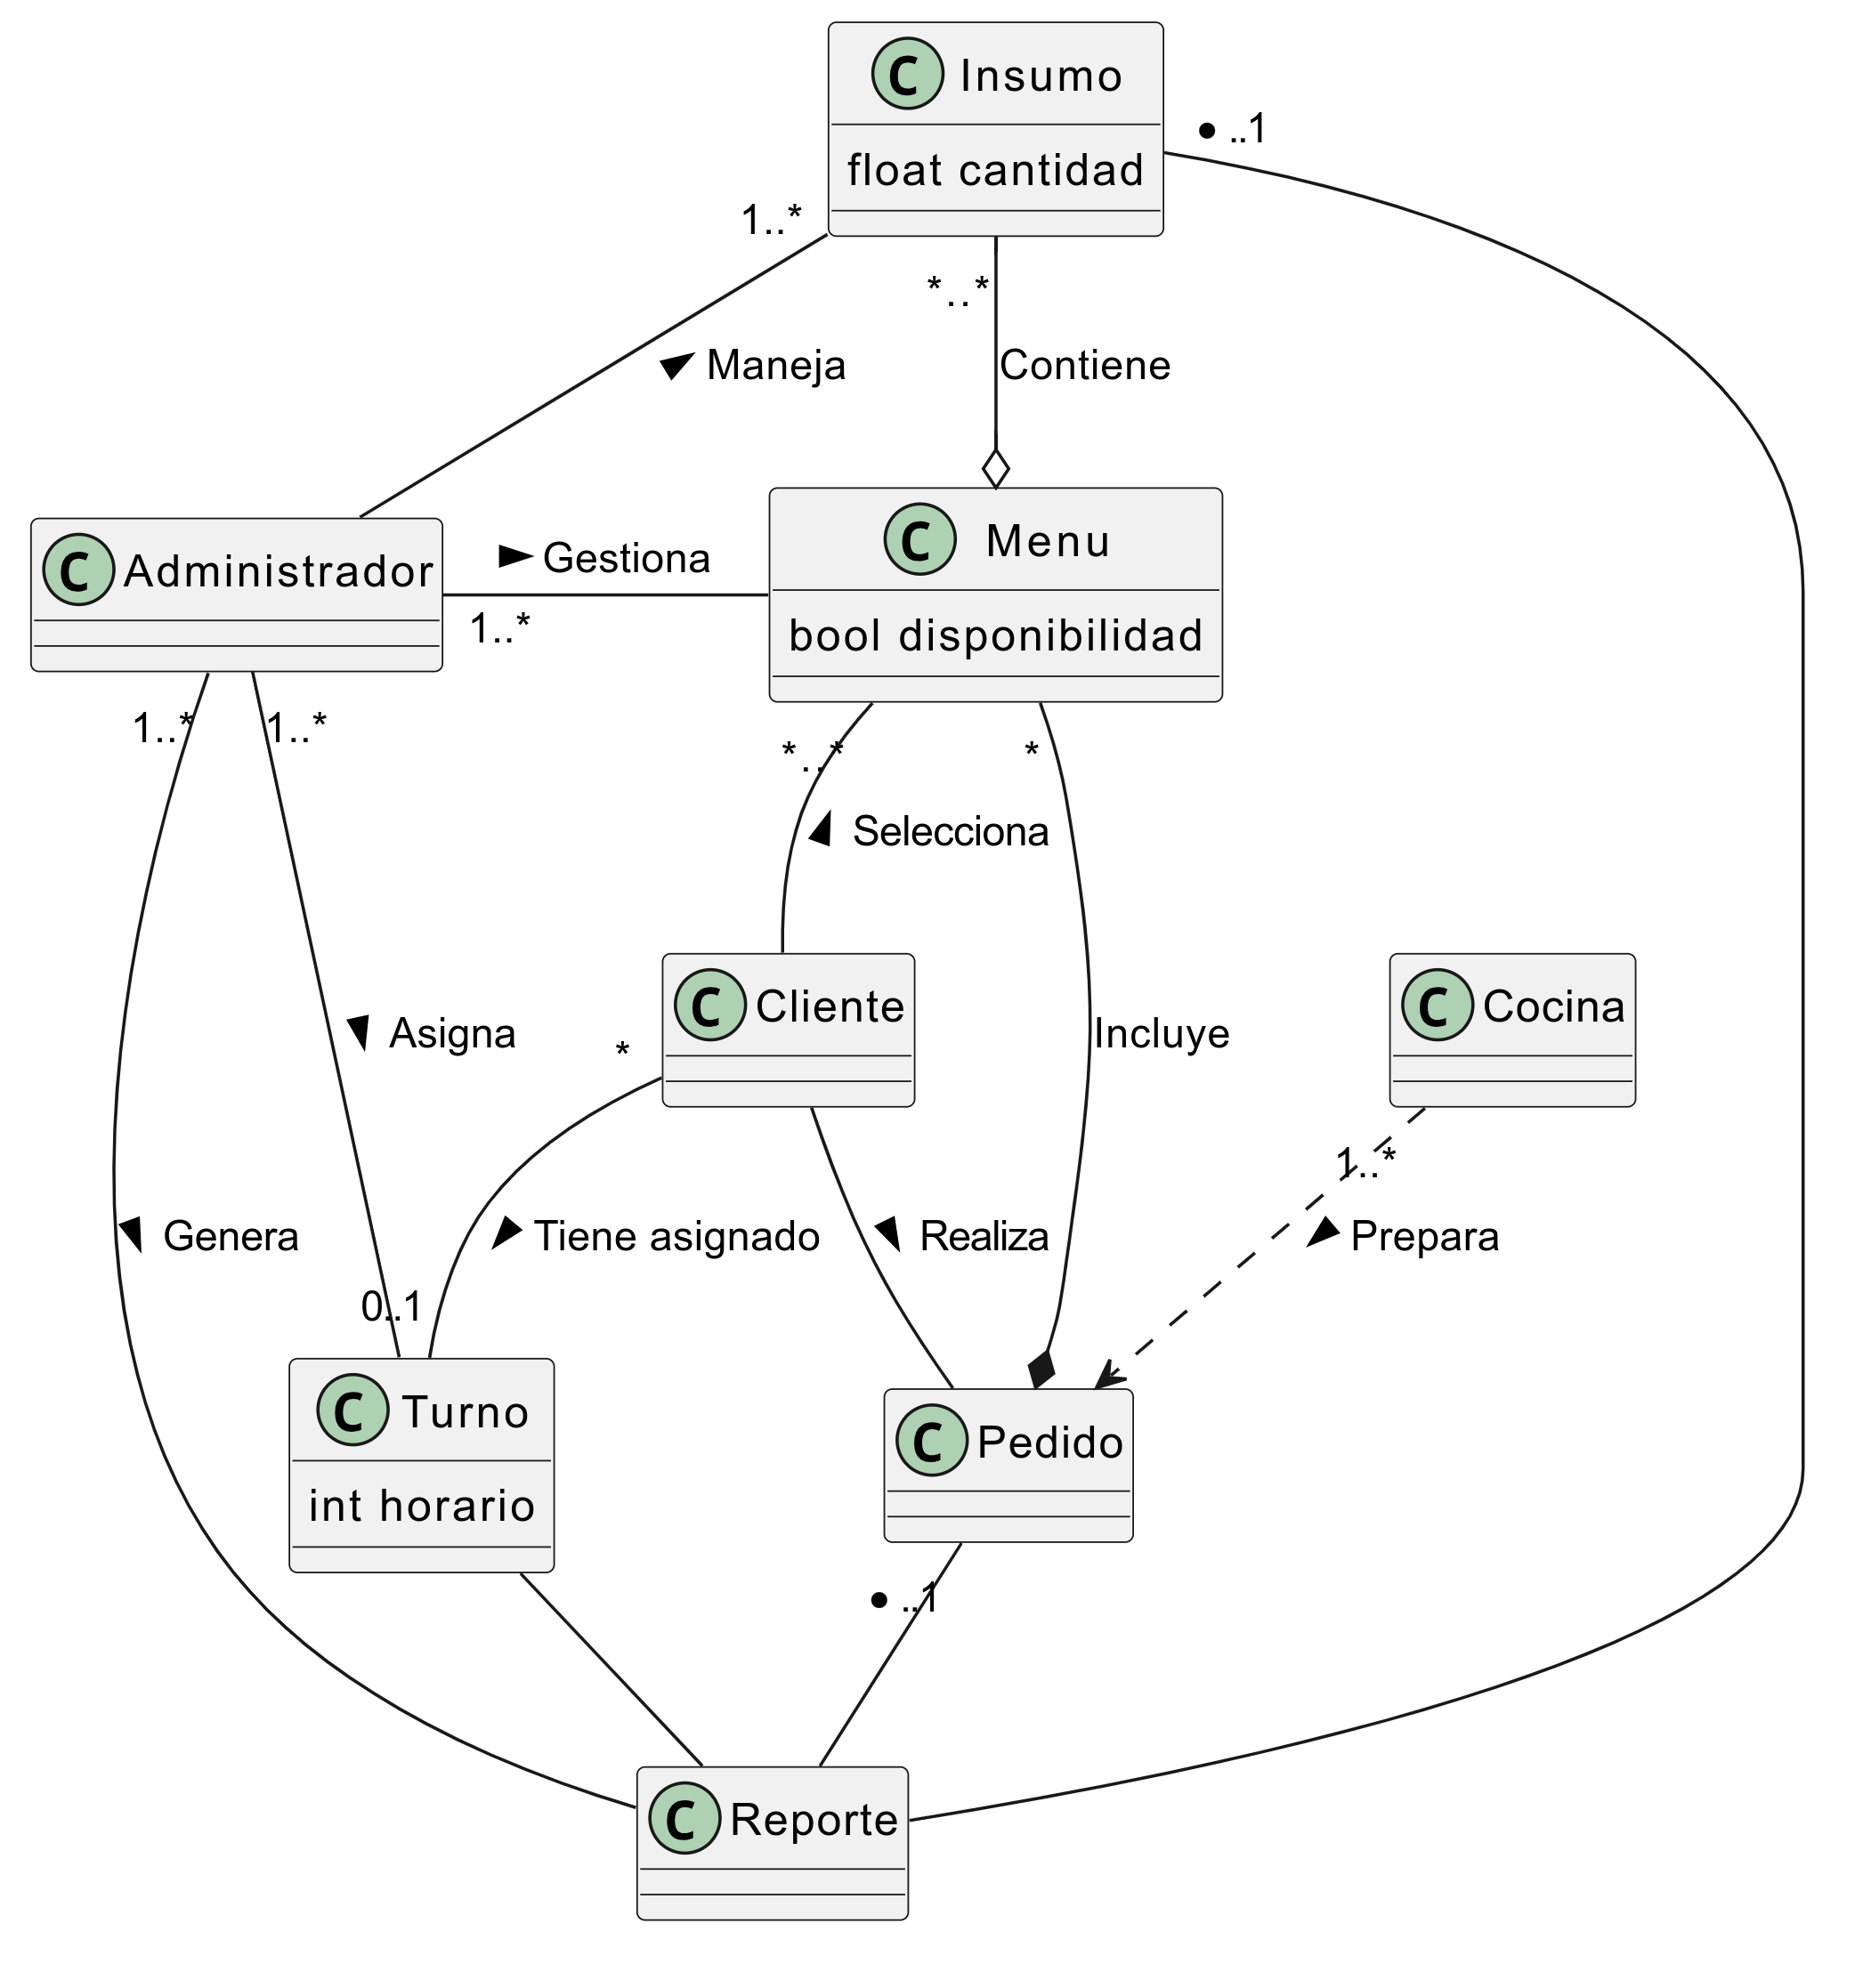
\includegraphics[width=15cm]{Domain Modeling [01] - Class Diagram.png}
\end{center}

\pagebreak

\section{Glosario de Términos}

\begin{itemize}
	\item \textbf{Cliente:} Persona que realiza y consume el pedido. Es el usuario final del servicio del comedor, quien selecciona los platos del menú. Puede realizar pedidos para consumir en el lugar o para llevar.
	\item \textbf{Administrador:} Persona que administra los insumos, reportes y turnos del comedor. Supervisa el inventario, organiza los horarios del personal y analiza los reportes para la toma de decisiones.
	\item \textbf{Trabajador:} Personal que opera en la cocina y otros espacios del comedor. Incluye cocineros, meseros y personal de limpieza. Trabajan en coordinación con el administrador para cumplir con las demandas diarias.
	\item \textbf{Cocina:} Espacio del edificio donde se preparan los pedidos. Aquí se transforman los insumos en recetas listas para servir.
	\item \textbf{Pedido:} Receta que se le ofrece al cliente para comer. Representa la unidad básica de consumo en el comedor.
	\item \textbf{Reporte:} Contienen análisis de demanda y planificación de recursos del comedor. Incluyen datos históricos y proyecciones para optimizar la operación. Ayudan a identificar tendencias y áreas de mejora. Son herramientas clave para la toma de decisiones del administrador.
    \item \textbf{Turno:} Periodo de tiempo asignado en el cual un estudiante o usuario puede acceder al comedor. Los turnos están predefinidos y organizados para distribuir a los usuarios de manera eficiente a lo largo del día. Su asignación busca evitar aglomeraciones y garantizar un flujo ordenado de personas.
	\item \textbf{Insumo:} Materia prima para realizar recetas. Incluyen alimentos, condimentos y otros materiales necesarios para la preparación de los pedidos. Deben ser gestionados cuidadosamente para evitar desperdicios y garantizar la frescura.
	\item \textbf{Menú:} Conjunto de recetas que se ofrecen a los clientes. Es diseñado para satisfacer diferentes gustos y necesidades alimenticias. Puede variar según la temporada o la disponibilidad de insumos.
	\item \textbf{Datos de usuario:} Información para distinguir los usuarios, en esencia serían Nombre, Apellido y N$^{\circ}$ de Cédula. Estos datos son necesarios para identificar y registrar a los clientes y empleados. Su manejo debe cumplir con las normativas de protección de datos.
	\item \textbf{Consumo diario:} Cantidad de pedidos que se realizaron en un día. Es un indicador clave para medir la demanda y el desempeño del comedor. Ayuda a planificar la producción y gestionar los insumos. También permite identificar patrones de consumo y ajustar el menú o los turnos en consecuencia.
\end{itemize}

\pagebreak

\section{Diagrama de Contexto}

\end{document}
